PID- regulatoren er en reguleringssløyfe som består av proporsjonalt, integrasjon og derivasjons-ledd. 
Reguleringssløyfen arbeider for å minke forskjellen mellom målt verdi og ønsket verdi.

\begin{figure}[htp]
    \centering
    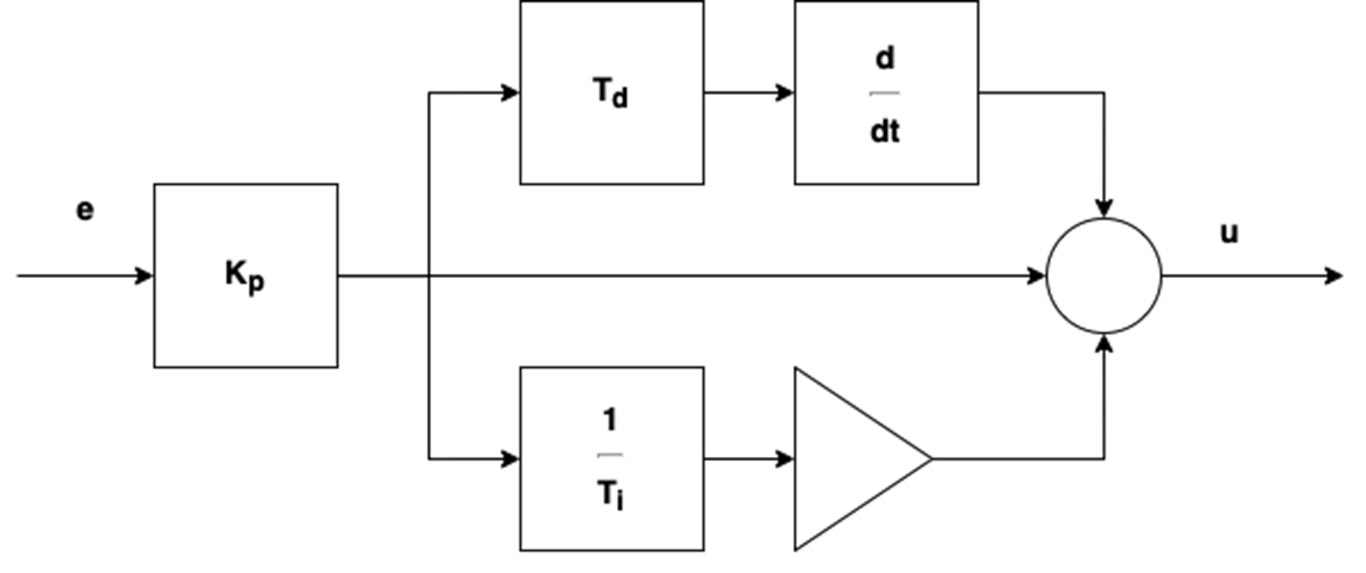
\includegraphics[width=0.7\columnwidth]{figures/reguleringssloyfe}
    \caption{PID-reguleringssløyfe.}
    \label{fig:reguleringssloyfe}
\end{figure}

\begin{itemize}
\item P: Proposjonalt ledd. $K_pe(t)$
\item I: Integrat ledd. $K_i \int_0^t e(t) dt$
\item D: Derivat ledd. $ K_d \frac{d e(t)}{dt} $
\end{itemize}

D-leddet gir pådrag gitt av akselerasjon.  D-leddet øker båndbredden til regulatoren slik hurtig regulering er mulig. 
Ved høye frekvenser kan d-leddet gi uønsket støy. Filtrering er ofte nødvendig for å fjerne støyen. \parencite{Balchen2000} 

\subsubsection{PID-regulering for droner}
For droner brukes PID regulatoren for å regulere rotasjon og posisjon til dronen. 
For å holde rotasjonen til dronen stabilt blir hver akse sin regulator justert for å minimere avvik. 
Dette kan være utfordrende å gjøre, analyse av logger og visuell inspeksjon av flyvninger kan hjelpe for å justere regulatorene.

Det er mulig å sette PID-regulator for å la dronen selv stabilisere seg. 
Her vil PID-regulatoren regulere hvor raskt og aggressiv dronen er for å rette opp rotasjonen. 
Mange droner har muligheten å sette dronen i Posisjon-hold modus. 
Denne funksjonen trenger PID-regulering for å bestemme hvor raskt og aggressivt dronen skal jobbe for å holde posisjonen. 

Transferfunksjon: 9.48
\[h_r(s) = K_p(1+\frac{1}{T_is}+T_ds) = K_p \frac{1+T_i(s)+T_iT_ds^2}{T_is} \approx K_p \frac{(1+T_is)(1+T_ds)}{T_is}\]

Filtrering
Støy. Statisk filter Dynamisk filter.
